\documentclass[border=6pt]{standalone}
\usepackage{tikz}
\usetikzlibrary{arrows.meta}
\begin{document}
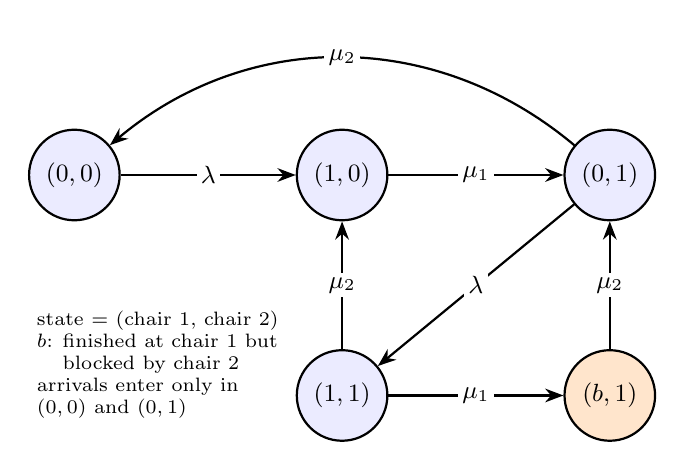
\begin{tikzpicture}[>=Stealth,font=\small,
 s/.style={draw,thick,circle,minimum size=1.15cm,inner sep=0pt,fill=blue!8},
 e/.style={->,thick},
 lab/.style={font=\small,fill=white,inner sep=1.5pt}]
\node[s] (00) at (0,0) {$(0,0)$};
\node[s] (10) at (3.4,0) {$(1,0)$};
\node[s] (01) at (6.8,0) {$(0,1)$};
\node[s] (11) at (3.4,-2.8) {$(1,1)$};
\node[s,fill=orange!20] (b1) at (6.8,-2.8) {$(b,1)$};
\draw[e] (00) -- node[lab]{$\lambda$} (10);
\draw[e] (10) -- node[lab]{$\mu_1$} (01);
\draw[e] (01) to[bend right=40] node[lab]{$\mu_2$} (00);
\draw[e] (01) -- node[lab]{$\lambda$} (11);
\draw[e] (11) -- node[lab]{$\mu_2$} (10);
\draw[e] (11) -- node[lab]{$\mu_1$} (b1);
\draw[e] (b1) -- node[lab]{$\mu_2$} (01);
\node[font=\scriptsize,align=left,anchor=north west] at (-0.6,-1.6) {state = (chair 1, chair 2)\\$b$: finished at chair 1 but\\\phantom{$b$: }blocked by chair 2\\arrivals enter only in\\$(0,0)$ and $(0,1)$};
\end{tikzpicture}
\end{document}
